\documentclass[uplatex,a4j,onecolumn,11pt,openany,english,oneside]{jsbook}
\usepackage{array,enumerate}
\usepackage[dvipdfmx]{graphicx,color}
\usepackage{amsmath}
\usepackage{bm}
\usepackage{amssymb}
\usepackage{comment}
\usepackage{algorithmic,algorithm}
\usepackage{otf}
\usepackage{float}
\usepackage{colortbl}
\usepackage{remreset}
\usepackage{ascmac}
\usepackage{multirow}
\usepackage{appendix}
\usepackage{url}
\usepackage{setspace}
\usepackage{subcaption}
\usepackage{tabularx}
\usepackage{lscape}
\usepackage{threeparttable}
\usepackage{caption}
\usepackage{booktabs}
\usepackage{longtable}
\usepackage{arydshln}
\usepackage{enumitem}   % 骨子段階のコンパクト表示用（本文化後も維持可）
\setlist{nosep, leftmargin=1.6em}
\captionsetup[table]{labelsep=period, labelfont=bf, justification=centering, singlelinecheck=off}
\captionsetup[figure]{labelsep=period, labelfont=bf, justification=centering, singlelinecheck=off}

% 図表を通し番号にする（テンプレート踏襲）
\makeatletter
	\@removefromreset{figure}{chapter}
	\def\thefigure{\arabic{figure}}
	\@removefromreset{table}{chapter}
	\def\thetable{\arabic{table}}
	\@removefromreset{equation}{chapter}
	\def\theequation{\arabic{equation}}
\makeatother
\setlength{\textwidth}{\fullwidth}
\setlength{\evensidemargin}{\oddsidemargin}
\setstretch{1.0}   % 骨子段階はコンパクト表示。本文化時に 1.3 へ戻す（テンプレート既定）

\newcommand{\argmax}{\mathop{\rm arg~max}\limits}
\newcommand{\argmin}{\mathop{\rm arg~min}\limits}

\renewcommand{\figurename}{Fig. }
\renewcommand{\tablename}{Table }
\renewcommand{\bibname}{References}
\renewcommand{\contentsname}{Contents}
\renewcommand{\prechaptername}{Chapter }
\renewcommand{\postchaptername}{}

\makeatletter
 \def\@cite#1{\textsuperscript{#1)}}
 \def\@biblabel#1{#1)}
\makeatother

\setlength{\abovecaptionskip}{0pt}
\setlength{\belowcaptionskip}{5pt}

% ===== 骨子段階のみ：章の強制改ページを抑制（本文化時にこのブロックを丸ごと削除） =====
\makeatletter
\renewcommand{\chapter}{%
  \par\vspace{1.2\baselineskip}%   % 改ページの代わりに縦スペース
  \plainifnotempty
  \global\@topnum\z@
  \if@english \@afterindentfalse \else \@afterindenttrue \fi
  \secdef
    {\@omit@numberfalse\@chapter}%
    {\@omit@numbertrue\@schapter}}
\makeatother
% ==================================================================================

\begin{document}
\thispagestyle{empty}
%%%%% 表紙 %%%%%
\begin{center}
\vspace*{3mm}
{\huge  修士論文}
\vspace{10mm}

{\huge Equation-Set Retrieval\\ Using Equations and Context\\ Extracted from the Literature\\ for Automated Physical Model Building\\}
\vspace{5mm}
{\LARGE 文献から抽出した数式と文脈を用いた\\
\vspace{5mm}
物理モデル自動構築のための数式集合検索}

\vspace{12mm}

{\huge ~指導教員　　加納　学　　教授}\\
\vspace{3mm}
\vspace{12mm}

{\huge 京都大学大学院情報学研究科}\\
\vspace{3mm}
{\huge システム科学専攻修士課程}\\
\vspace{3mm}
{\huge 令和 7 年度入学}\\
\vspace{30mm}

{\huge DING YIYANG}\\
\vspace{12mm}
{\huge 令和 9 年 2 月提出}
\end{center}

\newpage
%%%%% Abstract（2026-09-07 全章本文化後に書き直し。数値は第 6 章と同じ一次データ） %%%%%
\thispagestyle{empty}
{\huge \bf Abstract}
\\
\\
\\
\\
\\
Physical models underpin process design, control, and digital twins, but building one for a process outside the libraries of modeling tools requires an engineer to collect the equations scattered across many documents and to assemble them into a solvable system.
Our group aims to automate this work with an automated physical model builder (AutoPMoB).
This thesis addresses one of its steps: given a description of the desired model and its input and output variables, retrieve the set of equations that composes the model from an equation database built from multiple documents.
The answer is a set rather than a list --- a physical model is a system of equations that share variables and close with zero degrees of freedom --- so a candidate must be judged by its relation to the equations already selected, not by its relevance to the query alone.

We propose a two-stage retrieval method.
The first stage narrows the database by text similarity and variable overlap, and the second stage reranks the candidates with a multilayer perceptron that reads, beside seven query--equation features, three set-aware features that compare each candidate with the equations already selected: complementarity, coherence, and domain agreement.
A learned greedy variant builds the set one equation at a time, and a self-terminating criterion (DoF-stop) halts retrieval when the selected set closes as a system, so the method returns a solvable set without knowing the number of equations in advance.
To evaluate the method, we built a database of 11,146 equations from 361 sources and 2,838 test cases, 1,000 of which are synthesized closed systems whose answers are solvable by construction, and we split the sources so that no document leaks between training and testing.

% source: experiments/strat_A.json / strat_B.json（0.5206→0.7429, 0.4661→0.6890）;
%         external_baselines_stats.json（A ≤ 0.6020, B ≤ 0.5548）; llm_set_*_equiv_results.json
%         （0.2258–0.3003）; greedy_3way_stats.json; stage1_weight_stats.json（0.7799）;
%         dof_stop_stats.json（closed_dof 0.9363 / 0.8826 vs oracle 0.8651 / 0.7806）
The method raises Recall@K from 0.521 to 0.743 in the mixed setting and from 0.466 to 0.689 in the synthesized-only setting, on all 10 stratified splits; BM25 and dense retrieval with E5 stay at or below 0.602 and 0.555 even at their best mixing weights, and direct generation by a large language model reaches 0.23--0.30.
Analyses attribute the gain to the variables that equations share, whereas topical similarity becomes redundant once the first stage has screened the candidates.
Two interventions predicted by the analyses confirmed the mechanism: learned greedy selection recovered the saturation on the hardest cases, and a variable-weighted first stage raised Recall@K to 0.780.
DoF-stop returned closed systems for 94\% of the cases in the mixed setting and 88\% in the synthesized-only setting, more often than an oracle told the answer size.

\newpage
%%%%% 目次 %%%%%
\pagenumbering{roman}
\setcounter{tocdepth}{1}   % 骨子段階は章・節のみ。本文化時に 4 へ戻す
\tableofcontents
\thispagestyle{empty}
\newpage
\pagenumbering{arabic}
\chapter{Introduction}
\label{Introduction}
% ============================================================
% Chapter 1: Introduction — 本文（Phase 2, 2026-09-07）
% 骨子版（Phase 1, P1-P8）は git 履歴を参照。段落構成は骨子どおり:
%   P1 問題 / P2 AutoPMoB（図 1）/ P3 本研究の課題と「集合」の必然性（CSTR）/ P4 手法 /
%   P5 データと分割 / P6 結果 / P7 貢献 / P8 章構成
% 数値の一次ソースは各段落の % source: コメントに記載（2026-09-07 に JSON と照合）。
% 図 1 は generate_figures_thesis.py overview() で生成（figures/fig_autopmob_overview.pdf）。
% 設計書: docs/superpowers/specs/2026-09-07-w2-introduction-design.md
% ============================================================

Physical models --- systems of equations that describe how the material, energy, and momentum
of a process change --- underpin the process industry. Process design sizes equipment on them,
process control tunes controllers on them, and a digital twin keeps such a model in step with the
running plant\cite{DigitalTwin}. Purpose-built tools such as MATLAB/Simulink\cite{simulink} and
Aspen Plus\cite{aspen} let an engineer assemble a model quickly, but only for the unit operations
and phenomena that their libraries already cover. For a process outside those libraries, the
engineer surveys a large body of papers, textbooks, and handbooks, collects the equations
scattered across them, and refines a prototype model by trial and error. Modeling a new process
is therefore slow, and it depends on the few experts who can read the literature of the field.

To free engineers from this work, our group aims to develop an automated physical model builder,
AutoPMoB\cite{AutoPMoBCSTR,AutoPMoBProto}. Fig.~\ref{fig:overview}(a) shows its pipeline:
AutoPMoB collects documents about a target process, extracts equations, variables, and
experimental data from them, judges which extracted items are equivalent across documents, and
reorganizes the equivalent items into the desired model. Our group has developed its component
technologies step by step: an annotation tool and an extraction algorithm collect variable symbols
from engineering documents\cite{VARAT}, a language model pre-trained on a chemical-engineering
corpus judges whether two variable definitions refer to the same quantity\cite{ProcessBERT}, and
a computer-algebra algorithm judges whether two equation systems are
equivalent\cite{DAEEquiv}.

\begin{figure}[htb]\centering
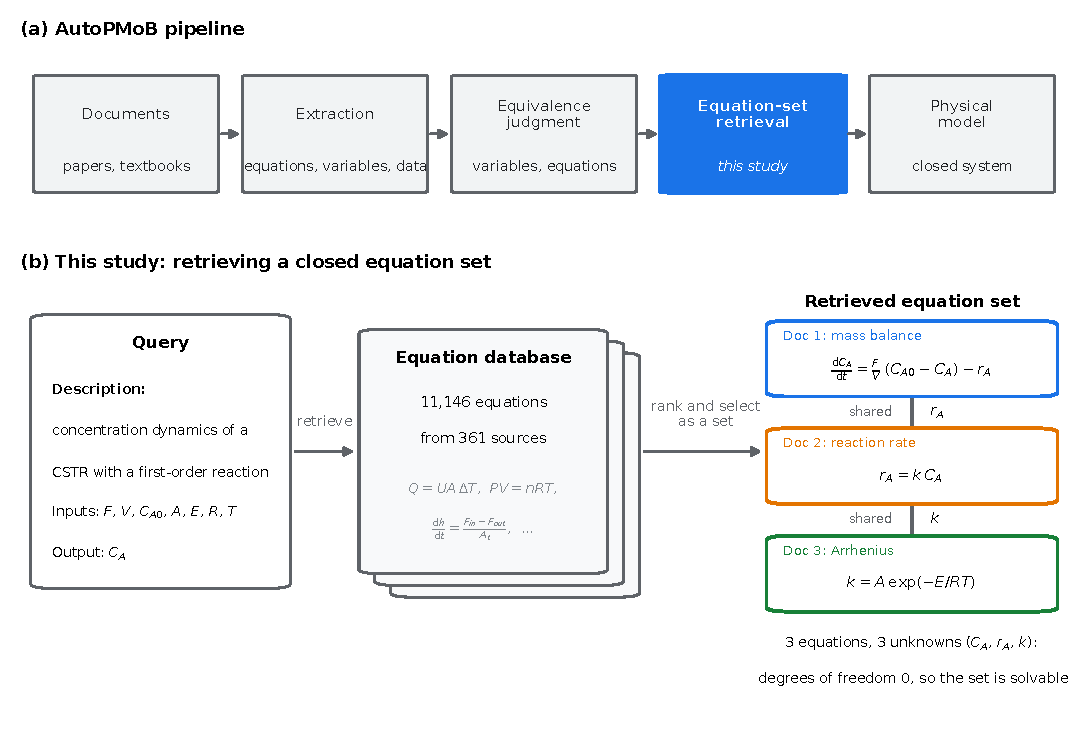
\includegraphics[width=0.98\linewidth]{figures/fig_autopmob_overview.pdf}
\caption{The automated physical model builder (AutoPMoB) and the position of this study. (a)
AutoPMoB collects documents about a target process, extracts equations, variables, and data,
judges their equivalence across documents, and reorganizes them into the desired model; this
study addresses the highlighted stage. (b) The task of this study: a query gives a description of
the desired model with its input and output variables, and the method retrieves, from a database
of 11,146 equations drawn from 361 sources, the set of equations that composes the model. The
three retrieved equations come from different documents and are linked by the variables they
share ($r_A$ and $k$); with three equations and three unknowns ($C_A$, $r_A$, and $k$) the set
has zero degrees of freedom, so a simulator can solve it.}
\label{fig:overview}
\end{figure}

This study addresses the reorganization step, the highlighted stage of
Fig.~\ref{fig:overview}(a): given a description of the desired model together with its input and
output variables, retrieve the set of equations that composes the model from an equation database
built from many documents (Fig.~\ref{fig:overview}(b)). The step is a retrieval problem with an
unusual answer. A physical model is not a list of independent equations but a system of equations
that share variables and must be solved simultaneously, and the system can be solved only when it
has as many equations as unknown variables --- when its degrees of freedom are zero --- so that,
once the inputs are given, every output is determined. The concentration dynamics of a continuous
stirred-tank reactor (CSTR), for example, need three coupled equations: the mass-balance ordinary
differential equation (ODE) for the concentration, the reaction-rate equation $r_A = k C_A$, and
the Arrhenius equation $k = A\exp(-E/RT)$ for the rate constant. The ODE alone leaves the rate
$r_A$ undetermined, the rate equation alone leaves the rate constant $k$ undetermined, and only
the three together close the system. A method that scores each equation by its similarity to the
description cannot see these dependencies: each of the three equations looks only moderately
relevant on its own, an equation from an unrelated document may look more relevant than any of
them, and no similarity score tells whether a set of equations closes. Retrieval must therefore
evaluate candidate equations as a set, not one by one.

We propose a two-stage retrieval method whose second stage evaluates each candidate against the
equations already selected. The first stage ranks the whole database by a mixture of text
similarity and variable overlap and keeps the top candidates. The second stage reranks the
candidates with a multilayer perceptron (MLP) that reads ten features per candidate: seven
features of the query--equation pair, such as the text similarity and the fraction of the query
variables the equation contains, and three set-aware features that compare the candidate with a
reference set --- the top-ranked candidates or, in the sequential variants, the equations already
selected. The set-aware features ask whether the candidate supplies query variables the reference
set still lacks (complementarity), whether it shares variables with the set (coherence), and
whether it comes from the same field (domain agreement). We further introduce a learned greedy
selection that builds the set one equation at a time and trains with teacher forcing so that
training and inference see the same sequential context, and a self-terminating criterion
that halts retrieval when the selected set closes as a system (DoF-stop, named after the degrees
of freedom it monitors). The method thus returns
a ranked, solvable equation set without being told how many equations the answer has.

To evaluate the method under realistic difficulty, we construct a large equation database and
test cases whose answers are solvable, and we split them so that no document leaks between
training and testing. The database holds 11,146 equations from 361 sources, extracted from the
documents by a large language model (LLM) and normalized in notation. The 2,838 cases fall into
three families by how their answer sets were formed --- as published in one document, assembled
across documents, or synthesized --- plus augmented copies used only for training; the 1,000
synthesized cases grow by a rule that adds variable-sharing equations until the system closes, so
their answers are solvable by construction. We assign every source wholly to training,
validation, or testing, and we stratify the assignment so that four difficulty-related
distributions match between training and testing. All experiments repeat over 10 random splits
and report the mean and the spread.
% source: unified_equations.json（11,146 式・361 source）; training_cases.json（original 92 /
%         multisource_* 731 / dae_* 1,000 / 拡張 1,015 = 2,838）; 第 4 章 §4.1-4.4

Experiments show that the proposed method outperforms lexical and dense retrieval baselines and
direct generation by an LLM, and the analyses explain why. Recall@K --- the fraction of the
ground-truth equations found within the top $K$ of the ranking, where $K$ is the size of the
ground truth --- rises from 0.521 to 0.743 in the mixed setting and from 0.466 to 0.689 in the
hardest, synthesized-only setting, a gain of $+0.22$ in both on all 10 splits (Wilcoxon
signed-rank test, $p = 0.00195$).
% source: experiments/strat_A.json / strat_B.json results.*.Recall@K_correct（0.5206→0.7429,
%         0.4661→0.6890）; significance_stats.json（p_wilcoxon 0.00195）
Stronger text scorers do not close the gap: BM25 and a dense sentence encoder (E5), each mixed
with the variable-overlap term at its best weight, reach at most 0.602 and 0.555 in the two
settings, and an LLM that writes the equations directly reaches 0.23--0.30 even when a separate
model judges mathematical equivalence.
% source: experiments/external_baselines_stats.json best_per_scorer（A: bm25 0.6008 / e5io 0.6020;
%         B: bm25 0.5548 / e5io 0.5439）; llm_set_A/B/full_equiv_results.json（0.2545 / 0.2258 /
%         0.3003）
The analyses locate the cause of the gain in the structure of the answer rather than in its
topic: the set-aware features that read shared variables --- complementarity and coherence ---
carry the set-aware gain, domain agreement adds nothing ($p = 0.98$), and permuting the
variable-overlap features of the trained model collapses its score while permuting the topic
features leaves it unchanged.
% source: experiments/feature_x_difficulty_stats.json overall_tests（reranker-7+Dom −0.0001,
%         p_wilcoxon 0.98）; pfi_results.json（GROUP_var +0.678 / GROUP_topic +0.006, p=0.10）
Two interventions then confirm the mechanism causally. The mechanism analysis predicted that a
fixed reference set saturates on the hardest cases, and learned greedy selection recovers exactly
there ($+0.056$ on cases with eight or more equations); the error analysis predicted that the
text-heavy first stage caps what the reranker can reach, and a variable-weighted first stage
raises Recall@K to 0.780. DoF-stop returns closed systems more often than an oracle that is told
the answer size (0.94 against 0.87 in the mixed setting and 0.88 against 0.78 in the
synthesized-only setting) while matching its exact-match rate.
% source: experiments/greedy_3way_stats.json tests_hard_X8plus train_vs_static（+0.056）;
%         stage1_weight_stats.json overall.reranker-10S w30-70（0.7799）;
%         dof_stop_stats.json closed_dof 0.8826 / 0.9363 vs closed_oracleK 0.7806 / 0.8651,
%         set_exact_dof = set_exact_oracleK（0.3678 / 0.5262）

The contributions of this thesis are threefold.
\begin{enumerate}
  \item A solvable-by-construction benchmark: an 11,146-equation database from 361 sources,
    1,000 synthesized cases whose equation sets close with zero degrees of freedom, and a
    stratified source-disjoint split with 10 seeds.
  \item A set-aware two-stage retrieval method that improves Recall@K by $+0.22$ over classical
    information retrieval, exceeds BM25, dense retrieval, and LLM direct generation, and, with a
    self-terminating criterion, returns a closed equation set without knowing the answer size.
  \item An empirical account of the mechanism --- which features cause the improvement, where
    it saturates, and where the remaining errors arise --- confirmed causally by two
    interventions, learned greedy selection and a variable-weighted first stage.
\end{enumerate}

The rest of this thesis is organized as follows. Chapter~2 reviews the component technologies of
AutoPMoB, information retrieval and reranking, direct generation by LLMs, and mathematical
information retrieval, and states how this study differs from each. Chapter~3 formulates the task
and presents the two-stage method, its sequential variants, and DoF-stop. Chapter~4 describes the
equation database, the construction of the test cases, and the stratified split. Chapter~5
defines the evaluation settings, the compared methods, and the metrics. Chapter~6 reports the
results and discusses them in the order performance, case characteristics, mechanism, a first
intervention, self-termination, the null result for topic similarity, error analysis, a second
intervention, and limitations. Chapter~7 concludes the thesis and outlines future work.

% \clearpage  % 骨子段階は連続レイアウト（本文化時に戻す）

\chapter{Related Work}
\label{RelatedWork}
% ============================================================
% Chapter 2: Related Work — OUTLINE (Phase 1)
% 各節末に必ず「本研究との相違」を置く（Kotoba Tech ルール）。
% ============================================================
\section{Component Technologies for Automated Physical Model Building}
\begin{itemize}
  \item \textbf{P1.} Automating physical model building requires a chain of component technologies, several of which have been developed in our group.
  \begin{itemize}
    \item Document collection, formula extraction, and variable-equivalence judgment (ProcessBERT\cite{ProcessBERT}) precede model assembly.
    % cite: 数式抽出・文書情報抽出の先行研究（Phase 2で実文献を検証して追加。捏造禁止）
    \item (difference) These works produce the equation database; this study addresses the downstream step of selecting a solvable equation set from it.
  \end{itemize}
\end{itemize}

\section{Information Retrieval and Reranking}
\begin{itemize}
  \item \textbf{P2.} Classical information retrieval ranks items independently by query--item relevance, and modern systems refine the top candidates with a second-stage reranker.
  \begin{itemize}
    % cite: TF-IDF/BM25 と retrieve-then-rerank の代表文献（Phase 2で検証して追加）
    \item Lexical methods (TF-IDF) and learned rerankers assume that item relevances are independent given the query.
    \item Diversification methods consider inter-item redundancy but not solvability.
    \item (difference) Our items are interdependent: a correct answer is a set that closes a system of equations, which motivates set-aware features.
  \end{itemize}
\end{itemize}

\section{Direct Generation of Domain Knowledge by Large Language Models}
\begin{itemize}
  \item \textbf{P3.} Large language models can generate domain equations directly from a description, which makes them a natural alternative to retrieval.
  \begin{itemize}
    % cite: LLMの科学知識生成・hallucination に関する代表文献（Phase 2で検証して追加）
    \item Generated equations may be physically valid yet differ in notation, and empirical equations with fitted coefficients are hard to reproduce verbatim.
    \item (difference) We use an LLM only as an external baseline (and for generating case descriptions); our method retrieves from a database, which keeps provenance and reproducibility.
  \end{itemize}
\end{itemize}

\section{Mathematical Information Retrieval}
\begin{itemize}
  \item \textbf{P4.} Mathematical information retrieval searches for single formulas similar to a query formula or text.
  \begin{itemize}
    % cite: math IR / formula search の代表文献（Phase 2で検証して追加）
    \item Existing systems rank individual formulas by structural or textual similarity.
    \item (difference) Our task returns a set of equations that jointly form a solvable model, a requirement absent from formula search.
  \end{itemize}
\end{itemize}

% \clearpage  % 骨子段階は連続レイアウト（本文化時に戻す）

\chapter{Set-aware Equation-Set Retrieval}
\label{Method}
% ============================================================
% Chapter 3: Set-aware Equation-Set Retrieval — OUTLINE (Phase 1)
% 特徴量定義の source: two_stage_query_conditioned.py compute_features (L212-236),
%                     set_aware_reranker.py docstring (gComp/gCoh/gDom) — 実装と一致させること
% ============================================================
\section{Problem Formulation}
\begin{itemize}
  \item \textbf{P1.} We formulate equation-set retrieval as ranking the equations in a database against a query that specifies the desired model.
  \begin{itemize}
    \item Query $q = (c, \mathcal{I}, \mathcal{O})$: a natural-language description $c$, input variables $\mathcal{I}$, and output variables $\mathcal{O}$.
    \item Database $\mathcal{E} = \{e_j\}$: each equation has its variable set $V(e_j)$, source document, and domain label.
    \item Ground truth: the equation set $\mathcal{R}_q \subset \mathcal{E}$ that composes the target model.
    \item Degrees of freedom of a selected set $S$: $\mathrm{DoF}(S) = |\mathrm{unknowns}(S)| - |S|$; the system is closed (solvable given the inputs) when $\mathrm{DoF}(S) = 0$.
    \item (wrap) The goal is to rank $\mathcal{R}_q$ at the top and, optionally, to return a closed set without knowing $|\mathcal{R}_q|$.
  \end{itemize}
\end{itemize}

\section{Stage 1: Candidate Retrieval with Query--Equation Features}
\begin{itemize}
  \item \textbf{P2.} The first stage scores each equation independently with seven query--equation features.
  \begin{itemize}
    % source: two_stage_query_conditioned.py compute_features L212-236（f0〜f6）
    \item (1) TF-IDF cosine similarity between the description and the equation text; (2) Jaccard similarity between the query I/O variables and the equation variables; (3) latent text similarity after singular-value decomposition (SVD); (4) input-variable coverage; (5) output-variable coverage; (6) fraction of the equation's variables that appear in the query I/O set; (7) binary domain match.
    \item The top-$k$ candidates by this score form the reference set for Stage 2.
    \item (wrap) Stage 1 is a strong classical-IR method on its own and serves as the baseline.
  \end{itemize}
\end{itemize}

\section{Stage 2: Set-aware Reranking}
\begin{itemize}
  \item \textbf{P3.} The second stage evaluates each candidate not in isolation but against a reference set, using three set-aware features.
  \begin{itemize}
    % source: set_aware_reranker.py docstring（gComp/gCoh/gDom の定義）
    \item Complementarity $g_{\mathrm{Comp}} = |V(e) \cap \mathcal{Q} \setminus \bigcup V(\mathrm{ref})| / |\mathcal{Q}|$: how many still-uncovered query variables the candidate supplies.
    \item Coherence $g_{\mathrm{Coh}} = |V(e) \cap \bigcup V(\mathrm{ref})| / |V(e)|$: how strongly the candidate shares variables with the reference set.
    \item Domain agreement $g_{\mathrm{Dom}}$: the fraction of the reference set that shares the candidate's domain.
    \item A multilayer perceptron (one hidden layer of 64 units, ReLU, dropout 0.1) scores the 10 features (7 + 3) and is trained with a pairwise ranking loss (margin 0.1).
    % source: experiments/strat_A.json config（hidden_dim 64, margin 0.1, loss pairwise）
    \item (wrap) We call this configuration reranker-10S.
  \end{itemize}
\end{itemize}

\section{Sequential Selection Strategies}
\begin{itemize}
  \item \textbf{P4.} Because set-aware features depend on what has already been selected, we compare three selection strategies.
  \begin{itemize}
    \item Static: set features are computed once against the fixed Stage-1 top-$k$ reference.
    \item Greedy at inference: after each selection, set features are recomputed against the already selected set; the model itself is trained statically.
    \item Learned greedy: the model is also \emph{trained} on sequential contexts with teacher forcing — during training the true partial set is given as the reference, so training matches inference.
    % source: set_aware_reranker.py --train-greedy, --greedy-train-cap 8
    \item (wrap) The comparison isolates the effect of matching the training condition to the inference condition.
  \end{itemize}
\end{itemize}

\section{Self-terminating Retrieval with Degrees of Freedom}
\begin{itemize}
  \item \textbf{P5.} Retrieval should stop by itself when the selected equations form a solvable system, rather than requiring the answer size $K$.
  \begin{itemize}
    \item DoF-stop keeps selecting greedily and stops when $\mathrm{DoF}(S) = 0$, i.e., when every non-input variable is determined by some equation.
    % source: set_aware_reranker.py --stop-dof（greedy_close）
    \item The returned set is closed by construction, which is exactly what a downstream simulator needs.
  \end{itemize}
\end{itemize}
% 手法パイプライン図（2段階＋greedy＋DoF停止）は Phase 2 で作成し §3.2 冒頭に挿入する。

% \clearpage  % 骨子段階は連続レイアウト（本文化時に戻す）

\chapter{Equation Database and Test Case Construction}
\label{Dataset}
% Chapter 4: Equation Database and Test Case Construction — outline inserted by Task 9 of docs/superpowers/plans/2026-07-12-master-thesis-phase1.md

% \clearpage  % 骨子段階は連続レイアウト（本文化時に戻す）

\chapter{Experiments}
\label{Experiment}
% Chapter 5: Experiments — outline inserted by Task 10 of docs/superpowers/plans/2026-07-12-master-thesis-phase1.md

% \clearpage  % 骨子段階は連続レイアウト（本文化時に戻す）

\chapter{Results and Discussion}
\label{ResultsAndDiscussion}
% Chapter 6: Results and Discussion — outline inserted by Task 11 of docs/superpowers/plans/2026-07-12-master-thesis-phase1.md

% \clearpage  % 骨子段階は連続レイアウト（本文化時に戻す）

\chapter{Conclusion}
\label{Conclusion}
% ============================================================
% Chapter 7: Conclusion — 本文（Phase 2, 2026-09-07）
% 骨子版（Phase 1, P1-P2）は git 履歴を参照。
% 構成: 何をしたか → 何が分かったか（貢献 3 点に対応）→ 限界と今後の課題 3 方向。
% 数値は第 6 章と同じ一次データ（% source: を参照）。第 1 段の再設計は A1 で実施済みのため
% 将来課題から外し、第 2 段落の介入として記した（ギャップ分析 W3）。
% 設計書: docs/superpowers/specs/2026-09-07-w3-conclusion-abstract-design.md
% ============================================================

This thesis formulated one step of automated physical model building as a retrieval problem and
solved it with a method that treats the answer as a set. Given a description of the desired model
and its input and output variables, the method retrieves, from a database of 11,146 equations
drawn from 361 sources, the equations that compose the model. Because a physical model is a
system of equations that share variables and close with zero degrees of freedom, the method
scores each candidate not only by its relevance to the query but by its relation to the equations
already selected: a first stage narrows the database by text similarity and variable overlap, and
a second stage reranks the candidates with a multilayer perceptron that reads three set-aware
features --- complementarity, coherence, and domain agreement --- beside seven query--equation
features. A learned greedy variant builds the set one equation at a time, and a self-terminating
criterion, DoF-stop, halts retrieval when the selected set closes as a system.

The thesis makes three contributions. First, it provides a benchmark on which a failure can be
attributed to the method: 1,000 of the 2,838 cases are synthesized by a rule that grows a closed
system from an ordinary differential equation, so a solvable answer exists by construction, and a
stratified source-disjoint split with 10 seeds measures generalization to unseen documents.
Second, the set-aware two-stage method raises Recall@K from 0.521 to 0.743 in the mixed setting
and from 0.466 to 0.689 in the synthesized-only setting, on all 10 splits; BM25 and dense
retrieval with E5 stay at or below 0.602 and 0.555 even at their best mixing weights, and direct
generation by a large language model reaches 0.23--0.30. Third, the thesis explains the gain
rather than only reporting it. Ablation and permutation importance agree that the variable
overlap between an equation and the query --- and, among the set-aware features, the two that
read shared variables --- carries the improvement, whereas topical similarity, informative over
the whole database, becomes redundant once the first stage has screened the candidates. Two
predictions drawn from this analysis were tested by intervention and confirmed: learned greedy
selection recovered the saturation of the static reference set on the hardest cases ($+0.056$
at eight or more ground-truth equations), and a variable-weighted first stage raised the
candidate coverage and, with it, the end metric to 0.780. DoF-stop returned closed systems for
94\% of the cases in the mixed setting and 88\% in the synthesized-only setting, more often than
an oracle told the answer size (87\% and 78\%), at the same exact-match rate.
% source: experiments/strat_A.json / strat_B.json（0.5206→0.7429, 0.4661→0.6890）;
%         external_baselines_stats.json best_per_scorer（A ≤ 0.6020, B ≤ 0.5548）;
%         llm_set_A/B/full_equiv_results.json（0.2258–0.3003）; feature_x_difficulty_stats.json /
%         pfi_results.json（変数系 +0.678 / 話題系 +0.006）; greedy_3way_stats.json
%         tests_hard_X8plus（+0.056）; stage1_weight_stats.json（0.7799）; dof_stop_stats.json
%         closed_dof 0.9363 (A) / 0.8826 (B) vs closed_oracleK 0.8651 / 0.7806, set_exact 同一

Three directions follow from the limitations of Section~\ref{sec:limitations}. First, learned
greedy selection still trains with teacher forcing, and the ranking errors that remain after the
two interventions --- equivalent equations from different documents and equations that determine
the wrong variable --- lie outside every current feature; scheduled sampling addresses the former,
and a feature that encodes which variable an equation determines addresses the latter. Second,
the evaluation is database-internal and the variable notation of the queries matches the
database; validation on real modeling tasks, including requests whose equations are absent from
the database or written in a different notation, will show how far the results carry. Third, the
method should be integrated into the AutoPMoB pipeline, downstream of equation extraction and
variable-equivalence judgment and upstream of a simulator, so that a retrieved closed set can be
solved and compared with plant data --- the test that automated model building must finally
pass.

% \clearpage  % 骨子段階は連続レイアウト（本文化時に戻す）

%%%%% References（2026-08-31 拡充: 30件。全件を一次ページで書誌確認済み・引用順） %%%%%
\begin{thebibliography}{99}

\bibitem{DigitalTwin}
F. Tao, H. Zhang, A. Liu, A. Y. C. Nee.
\ Digital Twin in Industry: State-of-the-Art.
\ {\it IEEE Transactions on Industrial Informatics}, {\bf 15}, pp.2405-2415, 2019.

\bibitem{simulink}
Simulink - Simulation and Model-Based Design - MATLAB \& Simulink.
\ \url{https://www.mathworks.com/products/simulink.html}.
\ (Accessed on 2026/07/12).

\bibitem{aspen}
AspenTech | Asset Optimization Software.
\ \url{https://www.aspentech.com/}.
\ (Accessed on 2026/07/12).

\bibitem{AutoPMoBCSTR}
S. Kato, M. Kano.
\ Towards An Automated Physical Model Builder: CSTR Case Study.
\ {\it Computer Aided Chemical Engineering}, {\bf 49}, pp.1669-1674, 2022.

\bibitem{AutoPMoBProto}
S. Kato, M. Kano.
\ Prototype of Automated Physical Model Builder: Challenges and Opportunities.
\ {\it Computer Aided Chemical Engineering}, {\bf 53}, pp.2839-2844, 2024.

\bibitem{VARAT}
S. Kato, M. Kano.
\ VARAT: Variable Annotation Tool for Documents on Manufacturing Processes.
\ {\it Journal of Chemical Engineering of Japan}, {\bf 58}, 2454461, 2025.

\bibitem{ProcessBERT}
S. Kato, K. Kanegami, M. Kano.
\ ProcessBERT: A Pre-trained Language Model for Judging Equivalence of Variable Definitions in Process Models.
\ {\it IFAC-PapersOnLine}, {\bf 55}, pp.957-962, 2022.

\bibitem{DAEEquiv}
S. Kato, C. Zhang, M. Kano.
\ Simple algorithm for judging equivalence of differential-algebraic equation systems.
\ {\it Scientific Reports}, {\bf 13}, 11534, 2023.

\bibitem{CombineEq}
S. Kato, M. Kano.
\ Automated physical model building from literature sources: Combining equations based on four predefined requirements.
\ {\it Computers \& Chemical Engineering}, {\bf 200}, 109147, 2025.

\bibitem{SINDy}
S. L. Brunton, J. L. Proctor, J. N. Kutz.
\ Discovering governing equations from data by sparse identification of nonlinear dynamical systems.
\ {\it Proceedings of the National Academy of Sciences}, {\bf 113}, pp.3932-3937, 2016.

\bibitem{ALAMO}
A. Cozad, N. V. Sahinidis, D. C. Miller.
\ Learning surrogate models for simulation-based optimization.
\ {\it AIChE Journal}, {\bf 60}, pp.2211-2227, 2014.

\bibitem{Manning}
C. D. Manning, P. Raghavan, H. Sch\"{u}tze.
\ {\it Introduction to Information Retrieval}.
\ Cambridge University Press, 2008.

\bibitem{Salton}
G. Salton, C. Buckley.
\ Term-weighting approaches in automatic text retrieval.
\ {\it Information Processing \& Management}, {\bf 24}, pp.513-523, 1988.

\bibitem{BM25}
S. Robertson, H. Zaragoza.
\ The Probabilistic Relevance Framework: BM25 and Beyond.
\ {\it Foundations and Trends in Information Retrieval}, {\bf 3}, pp.333-389, 2009.

\bibitem{LSA}
S. Deerwester, S. T. Dumais, G. W. Furnas, T. K. Landauer, R. Harshman.
\ Indexing by latent semantic analysis.
\ {\it Journal of the American Society for Information Science}, {\bf 41}, pp.391-407, 1990.

\bibitem{BERT}
J. Devlin, M. Chang, K. Lee, K. Toutanova.
\ BERT: Pre-training of Deep Bidirectional Transformers for Language Understanding.
\ {\it Proceedings of the 2019 Conference of the North American Chapter of the Association for Computational Linguistics: Human Language Technologies}, {\bf 1}, pp.4171-4186, 2019.

\bibitem{BERTrerank}
R. Nogueira, K. Cho.
\ Passage Re-ranking with BERT.
\ arXiv:1901.04085, 2019.

\bibitem{DPR}
V. Karpukhin, B. O\u{g}uz, S. Min, et al.
\ Dense Passage Retrieval for Open-Domain Question Answering.
\ {\it Proceedings of the 2020 Conference on Empirical Methods in Natural Language Processing}, pp.6769-6781, 2020.

\bibitem{LTR}
T. Liu.
\ Learning to Rank for Information Retrieval.
\ {\it Foundations and Trends in Information Retrieval}, {\bf 3}, pp.225-331, 2009.

\bibitem{MMR}
J. Carbonell, J. Goldstein.
\ The use of MMR, diversity-based reranking for reordering documents and producing summaries.
\ {\it Proceedings of the 21st Annual International ACM SIGIR Conference on Research and Development in Information Retrieval}, pp.335-336, 1998.

\bibitem{GPT3}
T. Brown, B. Mann, N. Ryder, et al.
\ Language Models are Few-Shot Learners.
\ {\it Advances in Neural Information Processing Systems}, {\bf 33}, pp.1877-1901, 2020.

\bibitem{LLMSR}
P. Shojaee, K. Meidani, S. Gupta, A. Barati Farimani, C. K. Reddy.
\ LLM-SR: Scientific Equation Discovery via Programming with Large Language Models.
\ {\it International Conference on Learning Representations}, 2025.

\bibitem{Hallucination}
Z. Ji, N. Lee, R. Frieske, et al.
\ Survey of Hallucination in Natural Language Generation.
\ {\it ACM Computing Surveys}, {\bf 55}, Article 248, 2023.

\bibitem{MathSurvey}
R. Zanibbi, D. Blostein.
\ Recognition and retrieval of mathematical expressions.
\ {\it International Journal on Document Analysis and Recognition}, {\bf 15}, pp.331-357, 2012.

\bibitem{NTCIR12}
R. Zanibbi, A. Aizawa, M. Kohlhase, I. Ounis, G. Topi\'{c}, K. Davila.
\ NTCIR-12 MathIR Task Overview.
\ {\it Proceedings of the 12th NTCIR Conference on Evaluation of Information Access Technologies}, pp.299-308, 2016.

\bibitem{ARQMath}
R. Zanibbi, D. W. Oard, A. Agarwal, B. Mansouri.
\ Overview of ARQMath 2020: CLEF Lab on Answer Retrieval for Questions on Math.
\ {\it Experimental IR Meets Multilinguality, Multimodality, and Interaction (CLEF 2020), Lecture Notes in Computer Science}, {\bf 12260}, pp.169-193, 2020.

\bibitem{Approach0}
W. Zhong, R. Zanibbi.
\ Structural Similarity Search for Formulas Using Leaf-Root Paths in Operator Subtrees.
\ {\it Advances in Information Retrieval (ECIR 2019), Lecture Notes in Computer Science}, {\bf 11437}, pp.116-129, 2019.

\bibitem{Hangos}
K. M. Hangos, I. T. Cameron.
\ {\it Process Modelling and Model Analysis}.
\ Academic Press, San Diego, 2001.

\bibitem{Gemini25}
G. Comanici, E. Bieber, M. Schaekermann, et al.
\ Gemini 2.5: Pushing the Frontier with Advanced Reasoning, Multimodality, Long Context, and Next Generation Agentic Capabilities.
\ arXiv:2507.06261, 2025.

\bibitem{ClaudeSonnet45}
Anthropic.
\ Introducing Claude Sonnet 4.5.
\ \url{https://www.anthropic.com/news/claude-sonnet-4-5}.
\ (Accessed on 2026/08/31).

\bibitem{ClaudeOpus48}
Anthropic.
\ Introducing Claude Opus 4.8.
\ \url{https://www.anthropic.com/news/claude-opus-4-8}.
\ (Accessed on 2026/09/07).

\bibitem{ClaudeFable51}
Anthropic.
\ Claude Fable 5.1.
\ \url{https://www.anthropic.com/claude/fable}.
\ (Accessed on 2026/09/07).

\bibitem{E5}
L. Wang, N. Yang, X. Huang, et al.
\ Text Embeddings by Weakly-Supervised Contrastive Pre-training.
\ arXiv:2212.03533, 2022.

\end{thebibliography}

%%%%% 謝辞（最終段階で執筆） %%%%%
%\newpage
%\chapter*{謝辞}

\newpage
\appendix
\def\thechapter{Appendix \Alph{chapter}}
% ============================================================
% Appendix — OUTLINE (Phase 1)
% 骨子段階は1章に統合（ページ節約）。本文化時に章分割を検討。
% ============================================================
\chapter{Supplementary Materials}

\section{Hyperparameters and Reproducibility}
% source: experiments/strat_A.json config / set_aware_reranker.py argparse defaults
\begin{table}[h]\centering
\caption{Hyperparameters of the reranker (identical across settings unless noted).}
\begin{tabular}{ll}
\toprule
Item & Value \\
\midrule
MLP hidden units / dropout & 64 / 0.1 \\
Loss / margin & pairwise ranking / 0.1 \\
Epochs / learning rate / batch size & 15 / 0.001 / 16 \\
Negative samples / weight decay & 8 / 0.0001 \\
Stage-1 top-$k$ & 50 (Settings A, B); 200 (greedy and DoF-stop runs) \\
Greedy training cap & 8 \\
BM25 baseline & $k_1 = 1.5$, $b = 0.75$, word unigrams \\
BM25 IDF & $\ln\{1 + (N - n + 0.5)/(n + 0.5)\}$ \\
E5 baseline & \texttt{intfloat/e5-base-v2}, mean pooling, $\ell_2$ norm \\
E5 maximum input length & 512 tokens \\
Text-score normalization (BM25, E5) & per-query min--max over the database \\
Equivalence judges (LLM baseline) & \texttt{claude-opus-4-8} (Table 3); \texttt{claude-fable-5-1} (check) \\
Random seeds & 42, 123, 456, 789, 1024, 2024, 3141, 5926, 7777, 9999 \\
\bottomrule
\end{tabular}
\end{table}

\section{Example of a Synthesized Case}
\begin{itemize}
  \item One synthesized case ($X=3$, CSTR) with its description, I/O variables, and ground-truth equations.
  % Phase 2: dae_cases.json から実例を1件転記する（改変しない）。
\end{itemize}

\section{LLM Prompts}
\begin{itemize}
  \item Prompts used for generating the descriptions of the synthesized cases and for the LLM direct-generation baseline, with pinned model identifiers.
  % Phase 2: generate_dae_cases.py / evaluate_llm_dae.py から実プロンプトを転記する（改変しない）。
\end{itemize}

\thispagestyle{empty}
\end{document}
